\chapter{Einführung}
In dieser Arbeit wird Anhand einer skizierten Situation eine Verhalndung nach dem "`Harvard-Konzept des Sachgerechten Verhandelns"'\cite{hk} weiter
HKSV bearbeitet. Die Einführungskapiteln werden ein kurzen Überblick geben über die Aufbau von HKSV\cite{hk} geben. Danach wird die Situtation
Analysiert anhand von Interessen von Parteien, folgend von entwickelten Entscheidungsmöglichkeiten (Optionen) und abschließend werden noch weitere Alternativen für Einigung
der Parteien vorgestellt. Fazit dieser Arbeit wird ein Überblick und die Ergebnise vorstellen.
\section{Harvard-Konzept des Sachgerechten Verhandelns}
Der nachfolgend dargestelltes Bild zeigt die Aufbau von HKSV\cite{hk}.
\begin{figure}[hb]
\centering
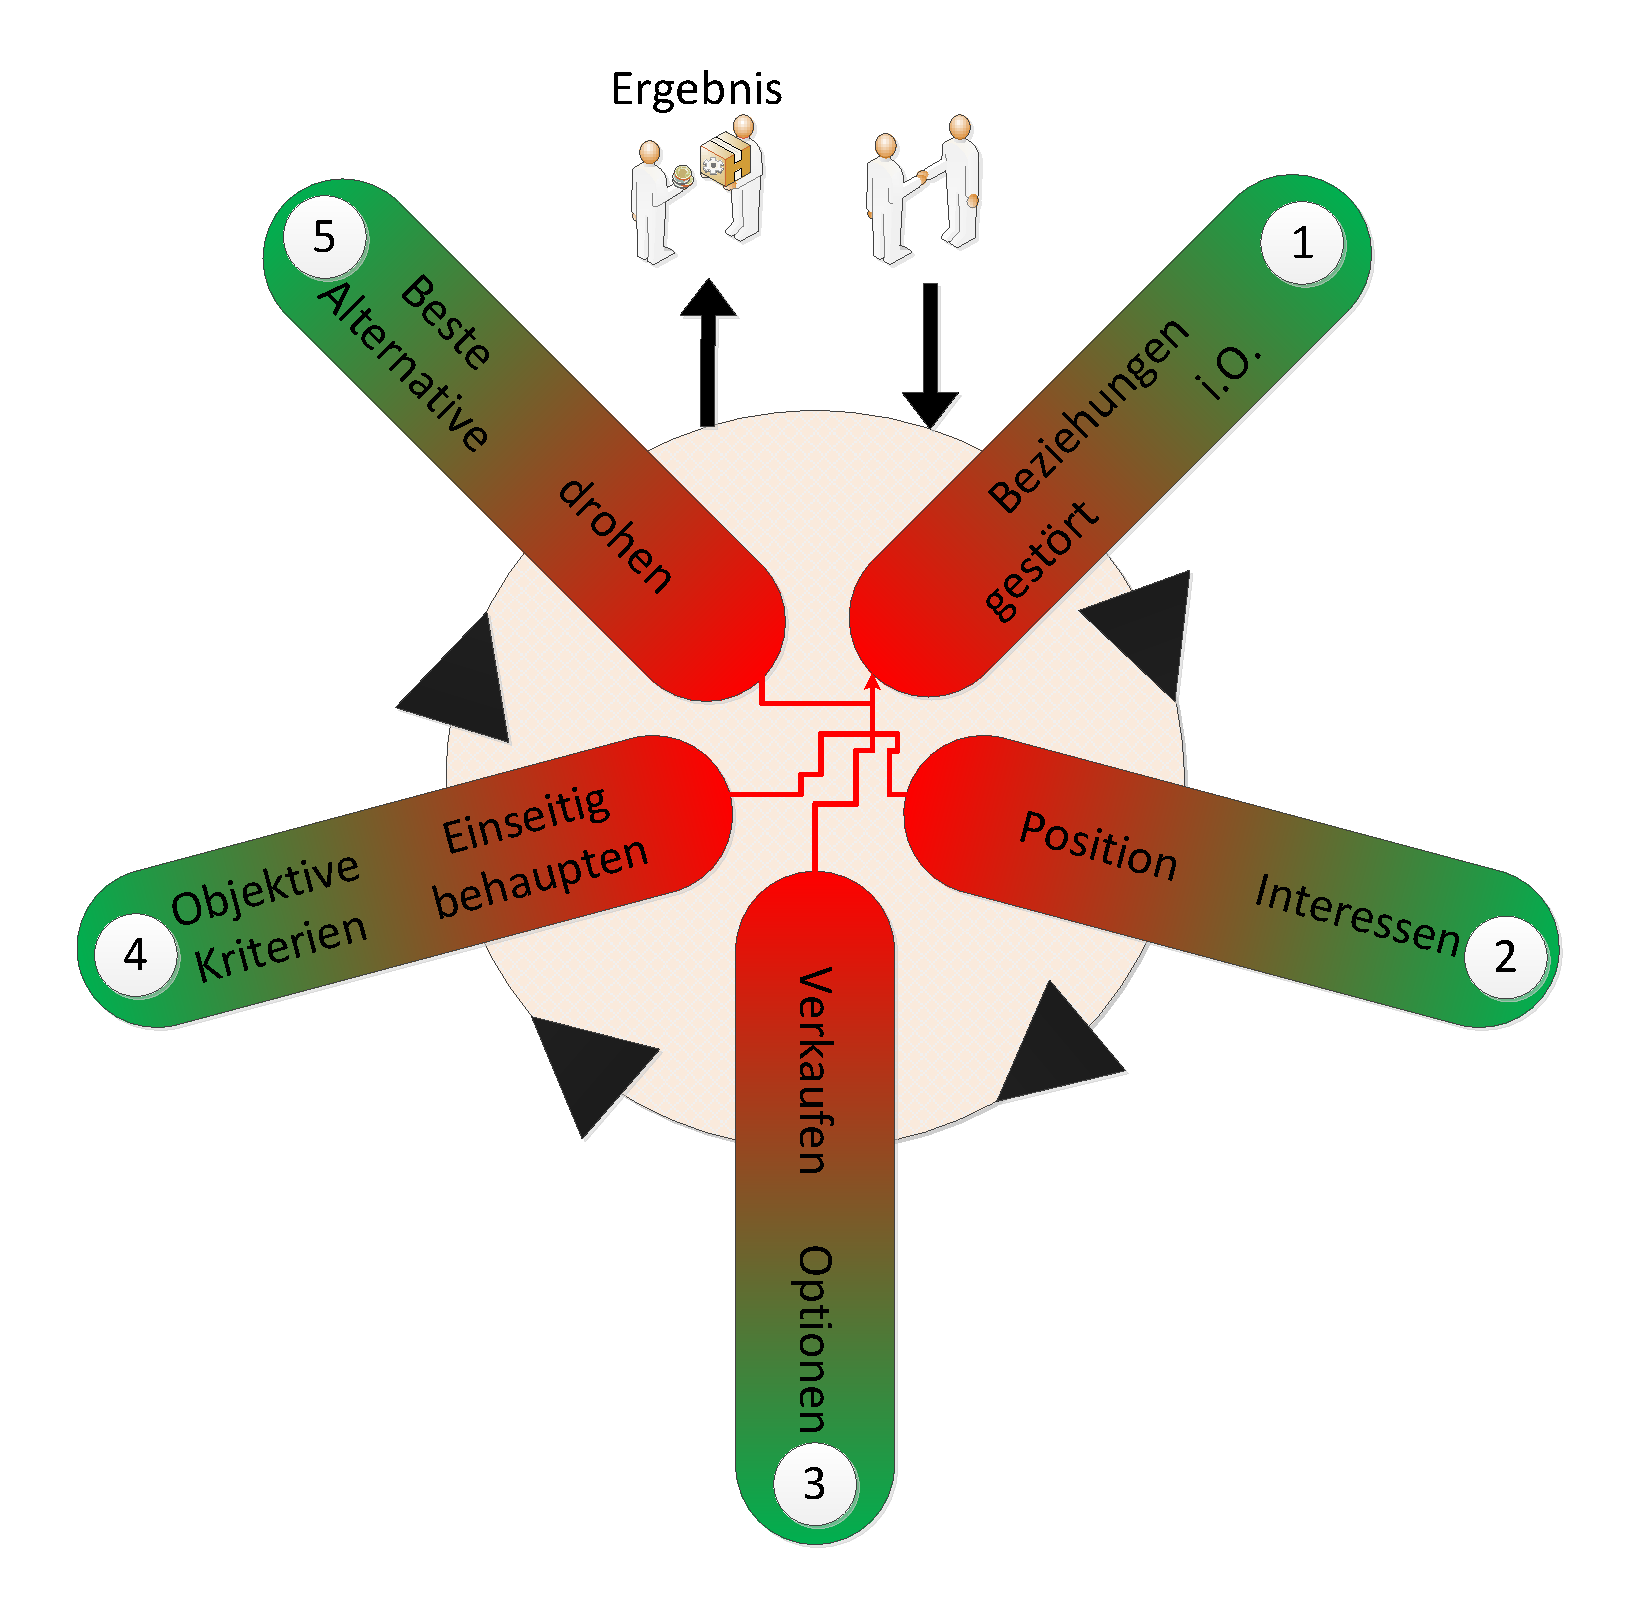
\includegraphics[width=0.4\paperwidth]{pictures/Harvard1}
\caption{Harvard-Konzept des Sachgerechten Verhandelns}
\end{figure}
Es sind die fünf Aspekte des Verhandelns zu erkennen, diese Beschreibt folgende Tabelle genauer. Die Punkte die in Bild mit Zahlen markiert sind
werden mit Stichwörtern markiert. Es wird verzichtet auf die genaueren Beschreibungen, da dies die Rahmen dieser Arbeit sprengen wird.
\begin{table}[h]
\begin{center}
\begin{tabular}{|l|l|l|}\hline
\textbf{Nummer} & \textbf{Name} & \textbf{Beschreibung} \\
\hline\hline
1 & Beziehungen & Trennung von Person und Sache \\
\hline
2 & Position vs Interessen & Interessenkonflikte, gemeinsame Interessen \\
\hline
3 & Verkaufen vs Optionen & Kreativität bei Lösungsstrategien \\
\hline
4 & Objektive Kriterien vs Behauptung & Ursachen, Standards, Werte \\
\hline
5 & Alternativen vs Drohungen & Alternativen für alle Beteiligten \\
\hline
\end{tabular}
\caption{Beschreibung von HKSV}
\label{tab:beschreibungHKSV}
\end{center}
\end{table}
Es ist wichtig nach dem HKSV zu erkennen, dass es mehrere Themen existieren die in roten Bereich gehen, wenn man sich auf diese währends Verhandelns
bewegt dann riskiert eine Partei, dass die Verhanldungen scheitern. Die Wechselseitige Wirkung wird durch die Bereiche gegenseitig verstärkt. \\
Nach diesem Konzept werden Heute sehr viele Verhandlungen durchgeführt und diese Idee ist gegenwärtig in Allen wichtigen Werken die über das Thema
Verhandlung behandeln.
